\chapter{First-order reversal curve diagram modelling of framboidal greigite}
\label{ch:res-4}
\fancyhead[L]{Chapter 5. FORC modelling of framboids}
\fancyhead[C]{}
\fancyhead[R]{}
\fancyfoot[C]{\thepage}

\section*{Abstract}
First-order reversal curve (FORC) diagrams are an increasingly used technique in rock magnetism that has the potential to identify magnetic domain state and magnetostatic inter-particle interactions. The hysteresis and FORC properties of non-interacting dispersions of greigite in the single-domain (SD) to single-vortex (SV) size range is well studied. However, most greigite occurs as highly interacting clusters. In this chapter, a micromagnetic method is used to study the FORC response of a simulated ensemble of highly interacting, close-packed greigite framboids. The magnetic signature of framboidal greigite is found to be very similar to that of multi-domain (MD) particles. Identification of MD-like FORC signals in samples known to contain greigite should be interpreted as produced by framboidal greigite.

\section{Introduction}
Greigite (Fe$_3$S$_4$) is a ferrimagnetic mineral often of authigenic origin in sediments \citep{Roberts2011}. It is most commonly found in strongly interacting, close-packed clusters called framboids \citep{Ariztegui1996,Rowan2006,Rowan2009,Roberts2011} (Fig. \ref{intro_01}).\par

The zero-field magnetic structure and stability properties of isolated greigite have been the subject of previous numerical studies (Chapter \ref{ch:res-1}; \citet{Muxworthy2013}). There have also been numerical simulations of the hysteresis and first-order reversal curve (FORC) properties of ideal single-domain (SD) grain (Chapter \ref{ch:res-2}) and single-vortex (SV) and SD grain (\ref{ch:res-3}) dispersions. However, the FORC properties of highly interacting ensembles of greigite is yet poorly understood.\par

In this chapter, a numerical micromagnetic finite element method (FEM) is employed to calculate the FORC response of a simulated ensemble of framboidal greigite composed of highly interacting, close-packed 30$\nm$ grains. At this size, these grains are SD in the non-interacing case (Chapter \ref{ch:res-3}) and produce FORC signals charactersitic of SD grains with cubic magnetocrystalline anisotropy (MCA) (Chapters \ref{ch:res-2},\ref{ch:res-3}).\par

Here, truncated-octahedral particles are chosen as the model geometry, because they are a common morphology for authigenic greigite \citep{Snowball1997,Roberts2011}. Also, truncated-octahedral solids can efficiently tessellate 3D space (the bitruncated cubic honeycomb) and thus produce the close-packed geometries observed in framboidal greigite.\par

Touching grains are theoretically problematic to model as possible exchange coupling between particles is not well understood. Here, a vanishing exchange coupling is assumed. Framboidal geometries with small gaps between the particles are used, so the only inter-particle interaction is magnetostatic.\par

Ferromagnetic materials have magnetisation states that are dependent on their magnetic (or thermal, chemical) history. This is the well-known phenomenon of magnetic hysteresis. Standard hysteresis measurements proceed by saturating the magnetisation by applying a saturating magnetic field $\boldsymbol{B}$ ($=\mu_0\boldsymbol{H}$) with strength $B_{\text{sat}}$; in this saturated state, magnetisations are uniform and completely aligned with the applied field. Gradually, the magnetic field strength is decreased to desaturate the magnetic material. A curve $M=M(B)$ of the projection of the material's magnetisation on the applied field direction $M=\boldsymbol{M}\cdot\boldsymbol{\hat{n}}$ (where $\boldsymbol{\hat{n}}$ is a unit vector in the direction of the applied field) against the applied field strength $B$ is traced. When the applied field is removed, the remanent magnetisation state is left. The ratio of the saturation remanent state magnetisation $M_{\text{RS}} \geq 0$ to the saturation magnetisation $M_{\text{S}}$ is one of the key magnetic hysteresis parameters \citep{Dunlop}. The applied magnetic field strength is then increased in the direction opposite the initial (effectively, making $B<0$): the applied field value at which a magnetisation $M=0$ state is obtained is called the coercivity, $B_\text{C}$. If from this state the field is taken back to zero, a magnetisation $M>0$ is obtained; however, there exists a field value $B_{\text{CR}}<B_{\text{C}}$, called the coercivity of remanence, from which a remanent $M=0$ state is obtained for $B=0$. These fields and the ratio $B_{\text{CR}}/B_{\text{C}}$ are key parameters characterising a hysteresis curve. To complete a hysteresis loop, the magnetisation is driven to a negatively saturated state and gradually returned to the initial positive saturation state. This traces the main (upper and lower) branches of a hysteresis loop.\par

A scatter plot of the ratio $M_{\text{RS}}/M_{\text{S}}$ against $B_{\text{CR}}/B_{\text{C}}$ is called a Day plot \citep{Day1977} and is one of the most common plots in rock magnetism \citep{Dunlop}. Although these basic magnetic hysteresis parameters can be useful to discern the magnetic domain state and magnetisation reversal mechanisms of magnetic systems, it has been argued recently that the Day plot can lead to erroneous interpretations \citep{Egli2014,Roberts2017}. It is logical that access to the interior of the hysteresis loop can reveal more information about magnetic behaviours, which is the basic idea behind the calculation of $B_{\text{CR}}$.\par

\section{Methodology}
\subsection{The micromagnetic method}
A ferromagnetic (in the broad sense, i.e., including ferrimagnetic behaviour) material has a Gibbs free-energy functional (excluding the effects of thermal fluctuations and magnetostriction) which can be written as \citep{Brown}:
\begin{equation}
E_\text{G} = \int_{\Omega} (\phi_{\text{exchange}} + \phi_{\text{anisotropy}} + \phi_{\text{stray}} + \phi_{\text{external}})\,\text{d}^3 \boldsymbol{r},
\end{equation}
where $\Omega$ is the ferromagnetic volume and $\text{d}^3 \boldsymbol{r}$ the volume differential, so integration is carried out over the ferromagnetic body. Here,
\begin{equation}
\phi_{\text{exchange}}=A|\nabla\boldsymbol{m}|^2,
\end{equation}
where $\boldsymbol{m}$ is the reduced (unitary) magnetisation vector and $A$ the exchange stiffness constant, is an expression providing a continuum approximation of the energy density due to quantum-mechanical exchange forces between atomic spins \citep{Landau1935}.
\begin{equation}
\phi_{\text{anisotropy}}=\frac{K_1}{2}\sum_{i\neq j}\gamma_i^2\gamma_j^2 + K_2\prod_i\gamma_i^2,
\end{equation}
where $\gamma_i$ denote the direction cosines and $K_1,K_2$ the first and second magnetocrystalline (MCA) anisotropy constants, respectively, is the MCA energy density for cubic-anisotropic ferromagnets. In terms of the reduced magnetisation vector components this has the form:
\begin{equation}
\phi_{\text{anisotropy}}=K_1(m_x^2m_y^2+m_y^2m_z^2+m_z^2m_x^2),
\end{equation}
where $K_2$ has been neglected since in the cubic anisotropy system we are assuming, $K_1$ is the dominant term at room temperature. The magnetic Gibbs free-energy associated with the magnetostatic self-interaction of the ferromagnetic body and the stray magnetic field $\boldsymbol{H}_{\text{stray}}$ it produces is given by \citep{Brown}:
\begin{equation}
\phi_{\text{stray}}=-\frac{\mu_0M_\text{S}}{2} \boldsymbol{m} \cdot \boldsymbol{H}_{\text{stray}}
\end{equation}
where $M_\text{S}$ is the saturation magnetisation and $\mu_0=4\pi \times 10^{{-}7}\,\text{T}\text{m}/\text{A}$ is the magnetic constant or vacuum permeability. Finally, the energy density due to the magnetostatic interaction of the ferromagnetic body and an external field $\boldsymbol{H}_{\text{external}}$ is:
\begin{equation}
\phi_{\text{external}}=-\mu_0 M_{\text{S}} \boldsymbol{m} \cdot \boldsymbol{H}_{\text{external}}.
\end{equation}

From thermodynamics, it is well known that under isothermal and isobaric conditions a system will be driven spontanteously toward an equilibrium state with locally minimal Gibbs free-energy. Micromagnetic algorithms aim to find the equilibrium magnetisation $\boldsymbol{m}$ by minimising the Gibbs free-energy functional \citep{Fischbacher2017}. Here, a modified gradient-descent method \citep{OConbhui2017} is used.\par

Numerical solutions require a discretisation of the spatial domain into a grid or mesh with a finite number of points on which numerical solutions are calculated. In FEMs, three-dimensional space is decomposed into tetrahedral pieces called finite elements with the vertices of these elements called the nodes. On each of the mesh nodes, a unit vector is initially defined to create an initial guess; the micromagnetic algorithm then attempts to minimise the magnetic Gibbs free-energy by variating the orientation of each of these vectors while ensuring they remain unitary. In micromagnetic theory \citep{Brown} there are some linearisations, which means that there should not be large variations in the direction of $\boldsymbol{m}$ between neigbouring nodes. For unconstrained micromagnetic models it is expected that the microstructure will contain nouniform structures at least to some degree. To model nonuniform structures it is sufficient that the spatial discretisation in the model is always smaller than the exchange length $l_\text{exch} = \sqrt{2A/\mu_0M_\text{S}^2}$ \citep{Rave1998}, which for greigite is $l_\text{exch} \approx 6.6\, \text{nm}$; a maximum element size of 5$\nm$ has been chosen for all the meshes. The non-local problem of calculating the stray field is handled via a hybrid finite-element/boundary-element formulation \citep{Fredkin1990}.\par

\subsection{The FORC model}
First-order reversal curves are a set of partial hysteresis curves obtained from magnetisation states on the upper branch of the hysteresis loop for different field values $B_a$ \citep{Mayergoyz1986}. For a given $B_a$ and $M(B_a)$, the field $B=B_b$ is increased to positive saturation to trace a magnetisation curve. This proceedure for a number of $B_a$ values creates a magnetisation function on two variables $M=M(B_a,B_b)$ for $B_b \geq B_a$. The FORC distribution $\rho$ is then defined as \citep{Roberts2000}:
\begin{equation}\label{forc distribution}
\rho = -\frac{\mu_0^2}{2}\frac{\partial^2 M}{\partial B_a \partial B_b}.
\end{equation}\par

It has been argued that, the FORC distribution is an empirical analog of the Preisach distribution which is well defined for magnetic systems that do not necessarily obey the strict conditions imposed by the Preisach model \citep{Mayergoyz1986}. Contour plots of the FORC distribution are called FORC diagrams and have been used increasingly as a proxy for the magnetic domain state and magnetic reversal behaviour of a variety of systems \citep{Pike1999,Pike2001,Roberts2000,Dumas2007,Egli2010,Egli2014,Biasi2016,Proenca2017,Zhao2017}.\par

Calculation of the FORC distribution (Eq. \ref{forc distribution}) is performed by least-squares fitting of a second degree polynomial surface $M(B_a,B_b)=a_0 + a_1 B_a + a_2 B_b + a_3 B_a B_b + a_4 B_a^2 + a_5 B_b^2 + e$, where $e$ is a collection of error terms, on a subgrid of the magnetisation function $M(B_a,B_b)$ including ($2\times\text{SF}+1$)$^2$ points in the vicinity of $(B_a, B_b)$ as determined by the smoothing factor SF \citep{Pike1999}. If the magnetisation is approximated in this manner, calculation of Eq. \ref{forc distribution} yields $\rho=-\mu_0^2 a_3 / 2$. Rotated $(B_b,\,B_a)$ axes, the so-called coercive field $B_c = (B_b - B_a)/2$ (not to be confused with the coercivity $B_\text{C}$) and interaction field $B_u = (B_a + B_b)/2$, respectively, are used for contour plots to produce FORC diagrams.\par

In an ensemble of randomly oriented particles, there are equal probabilities of finding particles with any orientation within an area element of the unit sphere. To simulate a randomly oriented dispersion of identical particles efficiently, it is necessary to obtain a number of applied field directions (equivalently, particle orientations with respect to the applied field) each of them representative of a given area on the unit sphere. Additionally all these areas should span the unit sphere or alternatively, in high symmetry particle scenarios, a section of the sphere which can recreate the particle geometry under rotation operations (Chapters \ref{ch:res-2}, \ref{ch:res-3}). Given the symmetry of the modelled framboidal cluster geometries (Fig. \ref{FIG_F01}) it is sufficient to simulate the effects of field orientations on the spherical triangle delimited by $(1, 0, 0), (a, a, a), (0, 0, 1)$, where $a=1/\sqrt{3}$. Then, the spherical triangle is subdivided into roughly equiareal triangle sub-units to obtain 85 triangular cells. Each cell represents a field orientation we obtain the FORC response for here, with the coordinates of the centre of the cell used as the direction of the field. The weighted average (using the cell area as the weight for each field direction) of all the FORC responses for each of these field orientations is the approximation to the total FORC response of the ensemble:
\begin{equation}
M(B_b, B_a)_{\text{total}} = \frac{\sum_i^{\text{cells}}M_i(B_b,B_a) A_i}{\sum_i^{\text{cells}}A_i},
\end{equation}
where $A_i$ is the area of cell $i$ and $M_i$ the FORC response of the framboid for field direction associated with cell $i$.
\begin{figure}
\centering
\includegraphics[width=0.4\textwidth]{research-4/figs/mesh_orientations_HD.pdf}
\caption[Framboidal mesh and field orientations]{Framboidal mesh and field orientations. Field orientations are obtained from a triangular mesh over the spherical triangle delimited by $(1, 0, 0), (a, a, a), (0, 0, 1)$, where $a=1/\sqrt{3}$. Given the symmetry of the cluster, this region contains all field orientations of interest. The framboid contains 65 truncated octahedral particles each with size $d=30\nm$. The small gap between the particles is $\roughly$2$\nm$.}
\label{FIG_F01}
\end{figure}\par

Since these calculations are computationally intensive, it is important to reduce further the amount of calculations. For each field orientation, the upper branch of the hysteresis loop is calculated. Most of the curve is traced by the sum of reversible motions of the magnetisations in each of the individual particles in the framboid. Therefore, FORCs need only to be calculated for $B_a$ field values for which at least one particle undergoes an irreversible rotation (switching) (Chapters \ref{ch:res-2}, \ref{ch:res-3}).\par

A saturating field $B_{\text{sat}}=250\mT$ and an external field rate of change of 2$\mT$ is used for all calculations. This means that for each field orientation we calculate 251 FORCs to obtain the FORC signal of a given cluster orientation.\par

\section{Results}
\subsection{The hysteresis and FORC response of framboidal greigite}\label{framFORC}
The FORC response is dependent on field orientation with respect to the framboid; all the 30$\nm$ particles have the same orientation. When the field is close to the isolated particle easy axis $<$111$>$, the hysteresis response of the framboid is saturated as low as $\roughly 50\mT$ (Fig. \ref{FIG_F02}a). Complex local interaction fields cause outer particles to coherently rotate to minimise the stray fields as the field is decreased. The remanent state is a double magnetic super-vortex with a low remanence $\roughly 0.1 \, M_\text{S}$ that is due to the effective magnetic flux-closure brought about by the super-vortex structures \citep{Harrison2002,Evans2006} (Fig. \ref{FIG_Frem}). All particles in the framboid remain in a SD state throughout the hysteresis and FORCs.\par

The FORC diagram for the easy axis-aligned applied field (Fig. \ref{FIG_F02}b) has a positive peak at $B_c\approx 80\mT$ roughly 5$\mT$ above the $B_u=0$ axis. A negative response of comparable magnitude is situated below and to the left of the distribution peak. The positive peak response corresponds to the large upward jumps experienced by the reversal curve starting at the lowest switching field $B_a\approx{-}80\mT$ as it approaches positive saturation (Fig. \ref{FIG_F02}a). The negative response is caused by irreversible switching of individual particles in the framboid on FORCs with higher $B_a$ values at $B_b\approx 75 \mT$. Most of the FORC diagram has a noisy appearance due to the complexity of individual particle responses caused by the local interaction fields. However, a large, continuous, positive response close to the $B_c=0$ axis is important as it was found for all field orientations.\par

When the applied field is close to a hard axis, the hysteresis and FORC response is very different. The hysteresis main branches are much more rounded, desaturating via reversible motion and experiencing the first irreversible switchings at roughly 150$\mT$ (Fig. \ref{FIG_F02}c) which are much smaller than the jumps for the easy axis-aligned applied field response (Fig. \ref{FIG_F02}a). The FORC diagram (Fig. \ref{FIG_F02}d) is dominated by signals close to the $B_c=0$ axis.
\begin{figure}
\centering
\includegraphics[width=0.8\textwidth]{research-4/figs/forcs_easy_hard.pdf}
\caption[FORCs for fields along an easy and a hard axis]{FORCs for greigite clusters with 30$\nm$ crystallites for fields along an easy (a, b) and a hard (c, d) axis. When the field is aligned close to an easy axis, there is a peak FORC response on the $B_u=0$ axis at $B_c\approx 80\mT$ (b). For fields close to the hard axis, the FORC response has a peak for $B_c\approx 10\mT$ (d).}
\label{FIG_F02}
\end{figure}\par

Averaging the response for all 85 field orientations results in a very smooth set of FORCs (Fig. \ref{FIG_F03}a). The remanence of the framboid ensemble is $M_\text{RS}/M_\text{S}\approx 0.1$ and the hysteretic coercivity $B_\text{C}\approx 5\mT$; compare this to the remanence and coercivity of a noninteracting ensemble of isolated SD greigite particles of the same size, $M_\text{RS}/M_\text{S}\approx 0.86$ and $B_\text{C}\approx 24\mT$, respectively (Chapter \ref{ch:res-3}). The magnetostatic interactions between the particles in the framboids cause large decreases in the remanence and coercivity. The saturating field for the framboid ensemble is roughly 150$\mT$.\par

The FORC diagram of the simulated ensemble of framboidal clusters (Fig. \ref{FIG_F03}b) is dominated by a large response roughly centered at ($B_c=10\mT,B_u=0$) and two lobes roughly at ($B_c=10\mT,B_u=\pm 40\mT$). These sources are part of a larger, continuous signal roughly in the rectangle defined by coordinates ($B_c=0,B_u={-}60\mT$), ($B_c=20\mT,B_u={-}60\mT$), ($B_c=20\mT,B_u=100\mT$), ($B_c=0,B_u=100\mT$). This is because the set of averaged FORCs are very smooth and do not experience sharp discontinuities on the path tho positive saturation; therefore, the signal is dominated by the differences in magnetisation values along the upper branch that serve as starting points for the FORCs.\par

The negative and smaller positive responses form a noisy region to the right of this rectangle. However, these are only $\roughly 20 {\%}$ the magnitude of the peak response at maximum on some very small regions, and most of it is less than $\roughly 10 {\%}$. The simulated FORC response of an ensemble of randomly aligned greigite framboids (composed of 30$\nm$ particles) is much lower per mass than the response of noninteracting, isolated 30$\nm$ grains: 25.6$\times 10^{{-}9}\,\text{m}^4\text{A}^{{-}1}\text{kg}^{{-}1}$ and 531.6$\times 10^{{-}9}\,\text{m}^4\text{A}^{{-}1}\text{kg}^{{-}1}$ (Chapter \ref{ch:res-3}) for the peak responses, respectively.
\begin{figure}
\centering
\includegraphics[width=\textwidth]{research-4/figs/remanent_supervortex.pdf}
\caption[Framboid remanent super-vortex states]{Framboid remanent super-vortex states. Super-vortex structures are the remanent state for all field orientations. Shown here: (a) field close to an easy axis; (b) field close to a hard axis; (c) field close to a saddle point; (d) field close to an intermediate direction between the easy, hard and saddle point directions. The net magnetic moment of the ensemble is $\roughly 12^{\circ}$ from the applied field.}
\label{FIG_Frem}
\end{figure}\par

Using the model of Chapter \ref{ch:res-3}, the FORC response of noninteracting ensembles of isolated greigite particles in the size range 30--80$\nm$ is obtained to produce FORC diagrams of mixtures of framboidal greigite and isolated particles in the SD and SV magnetic domain states. FORC diagrams of mixtures of equal mass framboidal and noninteracting SD particles (30--48$\nm$) (Fig. \ref{FIG_F04}a) and equal mass framboidal and noninteracting SV particles (70--80$\nm$) (Fig. \ref{FIG_F04}b) are presented.
\begin{figure}
\centering
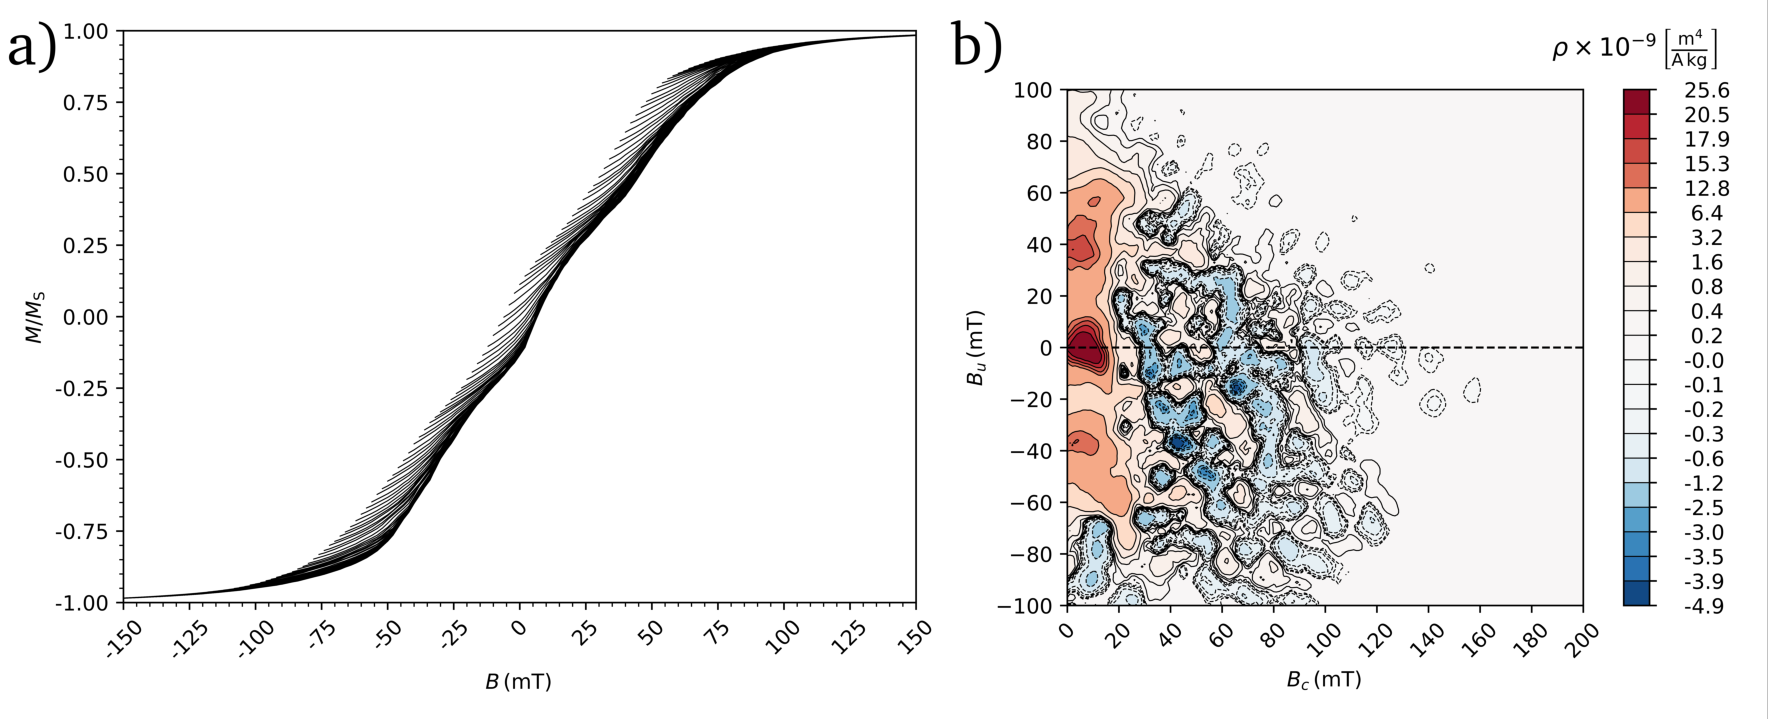
\includegraphics[width=\textwidth]{research-4/figs/forc_avg.pdf}
\caption[FORCs of the framboid dispersion]{FORCs of the greigite framboid dispersion. The framboids are formed by 65 particles identically aligned and with equal size $d=$30$\nm$. Averaging over the 85 field directions, the raw hysteresis/FORCs are smooth (a). The FORC response (b) is MD-like.}
\label{FIG_F03}
\end{figure}\par

The mixture of framboidal greigite and noninteracting SD particles (Fig. \ref{FIG_F04}a) is dominated by the noninteracting SD signal, erasing most of the noisy structure while keeping the important framboidal source close to the $B_c=0$ axis. When noninteracting SV particles are included (Fig. \ref{FIG_F04}b) to the framboid signal, the response is dominated by the SV particles. As with the mixture of SD and framboidal greigite, most of the noisy region disappears on account of it being so faint and there is more behaviour in the region close to the $B_c=0$ axis as SV particles' response is also in this region (Chapter \ref{ch:res-3}).
\begin{figure}
\centering
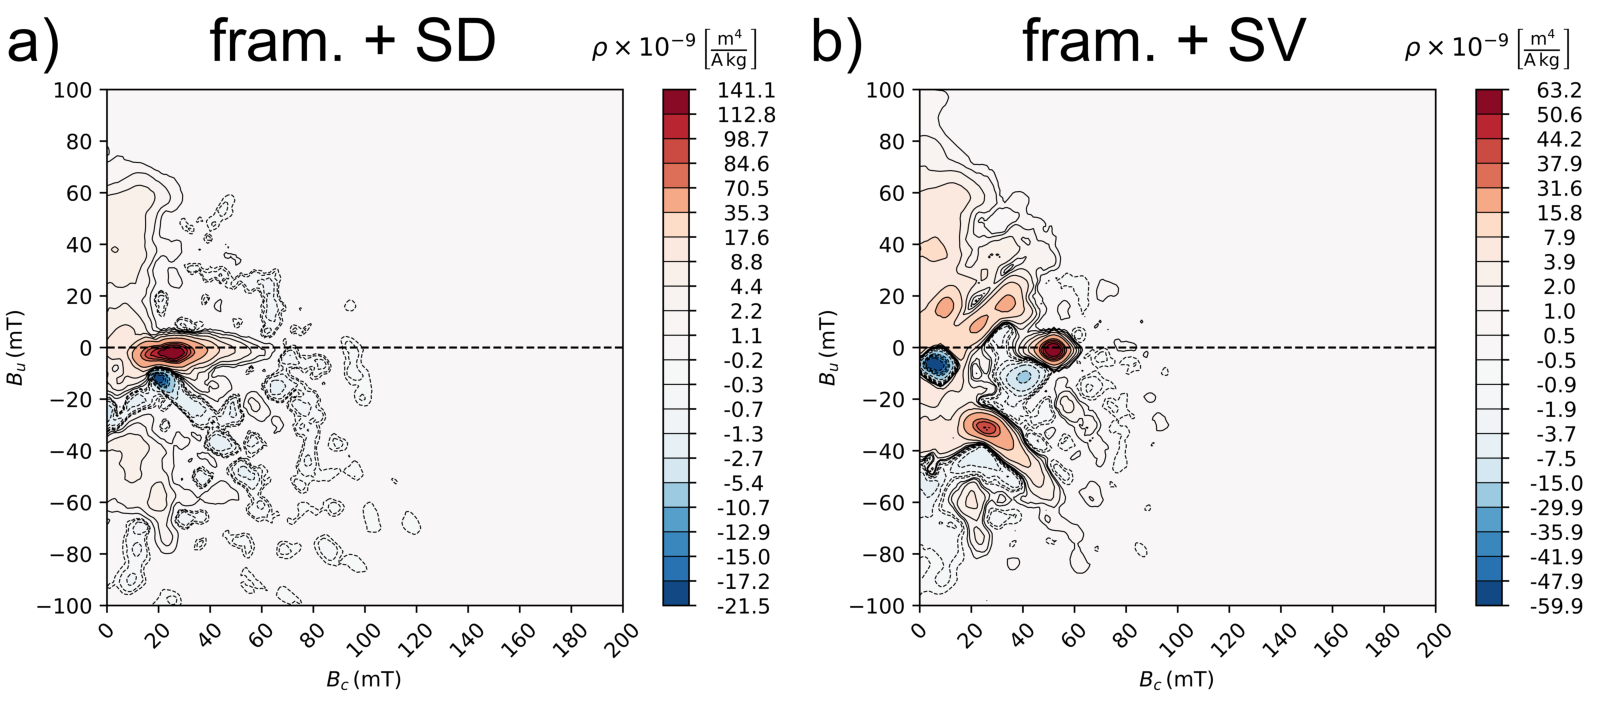
\includegraphics[width=\textwidth]{research-4/figs/forc_mix.pdf}
\caption[FORCs of a dispersion of framboids and non-interacting particles]{FORCs of a dispersion of equal-mass framboids and non-interacting SD (a) and SV (b) particles. The signal is dominated by the non-interacting particles because the framboid signal is weaker per unit mass. The framboid signal is still visible, however, as it occupies regions the non-interacting particles do not.}
\label{FIG_F04}
\end{figure}
\par

A scatter plot of the remanence of saturation $M_\text{RS}/M_\text{S}$ against the coercivity of remanence $B_\text{CR}$ to coercivity $B_\text{C}$ ratio, (Day plot \citep{Day1977}), reveals the simulated ensemble of framboidal greigite in a region that is unoccupied by the noninteracting, isolated particles (Fig. \ref{FIG_F05}), i.e., a region with a remanence as low as that of ensembles of SV particles $\roughly 80\nm$ but $B_\text{CR}/B_\text{C}$ values that are expected of smaller particles $\roughly 70\nm$ (Chapter \ref{ch:res-3}). Increasing content of SD or SV noninteracting particles have very different effects on the Day plot (Fig. \ref{FIG_F05}): increasing the SD content increases the remanence and decreases the $B_\text{CR}/B_\text{C}$ ratio; whereas, increasing the SV content has little effect on the remanence while increasing the $B_\text{CR}/B_\text{C}$ value.\par
\begin{figure}
\centering
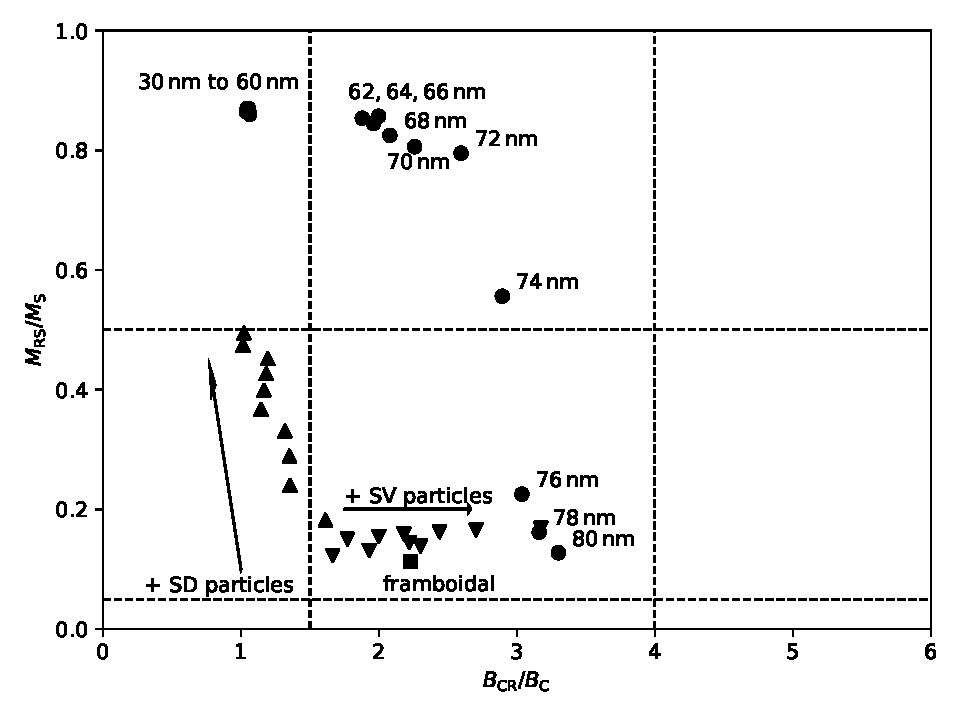
\includegraphics[width=0.6\textwidth]{research-4/figs/DayPlot.pdf}
\caption[Day plot of framboid and noninteraring particles mixtures]{Day plot of framboid and noninteraring particles mixtures. The framboidal clusters (square) plots in a region with very low $M_\text{RS}/M_\text{S}\approx 0.1$ and $B_\text{CR}/B_\text{C}\approx 2.2$. Increasing non-interacting SD particles content increases $M_\text{RS}/M_\text{S}$ and reduces $B_\text{CR}/B_\text{C}$. With increasing non-interacting SV particles content, the effect is to increase $B_\text{CR}/B_\text{C}$.}
\label{FIG_F05}
\end{figure}
\par

\subsection{Hysteresis of larger particle framboids}
An attempt was made to investigate FORC diagrams for assemblages of particles which are SV when isolated, however, due to memory and time constraints, the FORC response of larger particle framboids could not simulated. Instead, to investigate this, hysteresis simulations of framboids composed of fifteen (compared to 65 particles in Section \ref{framFORC}), larger SV particles with size $d=76\nm$ particles were carried out for a few selected field orientations. When the applied field is close to the easy axis the main branches remain saturated down to 50$\mT$ (Fig. \ref{FIG_F06}). As the field is decreased below this value, outer particles in the framboid nucleate hard-aligned vortices (Fig. \ref{FIG_F06}a). The remanent state (Fig. \ref{FIG_F06}b) has a super-vortex structure in which most particles are individually in a two-domain state with very clearly defined domain walls (Fig. \ref{FIG_F06}b, green). This state is remarkably similar to the easy-aligned SV state exhibited by large $>$200$\nm$ particles (Chapter \ref{ch:res-1}) with six easy aligned domains curling around the vortex core. However, in this super-vortex structure, outer particles are in a two-domain state and the six easy aligned magnetic domains span multiple particles. Non-interacting 76$\nm$ particles nucleate vortices (Chapter \ref{ch:res-3}); however, for this field orientation, the innermost particle in the cluster always remains in a SD state due to the internal magnetostatic interactions (Fig. \ref{FIG_F06}b, grey line). This is likely true for larger assemblages as the interaction fields deep inside the framboids will be stronger, thus favouring SD configurations for larger fractions of the crystallites in the framboid. This means that, for larger framboids composed of larger crystallites, the FORC signal could be very similar to the signal of framboids composed of SD crystallites (Section \ref{framFORC}).\par

\section{Discussion}
The FORC response of a framboidal cluster depends strongly on the orientation of the framboid relative to the applied field. When the field is aligned with an easy axis ($<$111$>$) the signal has its peak on the $B_u=0$ axis at $B_c \approx 80\mT$ (Fig. \ref{FIG_F02}b) and a vertical, almost-continuous feature centered on $B_c \approx 10\mT$ from $B_u \approx {-}60\mT$ to $B_u \approx 60\mT$. The latter bears similarities with FORCs calculated by \citet{Pike2001} for one-dimensional domain-wall pinning.\par

Remanent states for all particle-field configurations are super-vortex states (Fig. \ref{FIG_Frem}). For framboids formed by SD particles, the magnetic domain state of all individual particles in a framboid is SD; this probably holds for the innermost particles in larger framboids formed by larger SV particles. In the remanent state, the SD particles align in super-vortex configurations to create flux-closures, giving each framboid a very low net magnetic moment. This means that inter-framboidal interactions are weak even in cases when there are multiple framboids close to each other. The zero-field net magnetic moment of the simulated ensemble of framboids deviates from the applied field by $\roughly 12^{\circ}$. Whether framboidal greigite can carry potentially meaningful palaeo-directions is dubious. Simulations with more framboidal clusters and studies of the stability of the remanence could resolve this.\par

The FORC response of the simulated ensemble of clustered greigite (Fig. \ref{FIG_F03}) is very different from that of isolated SD and SV grains (Chapter \ref{ch:res-3}). Isolated SD greigite particles produce FORC signals with a characteristic boomerang shape, strong $B_u=0$ contributions and a tilted negative ridge. SV grains produce a more disjointed pattern. For isolated SD and SV grains the FORC response is dominated by irreversible switching which is evident in the raw hysteresis/FORC data. For framboidal greigite, the ensemble raw data is very smooth, i.e., there are no obvious discontinuities associated with irreversible events. This signal is very similar to MD signals \citep{Pike2001}.\par

Simulated FORC responses for ensembles of framboidal and isolated SD grains (Fig. \ref{FIG_F04}a) are very similar to those of framboid-rich samples obtained by \citet{Rowan2009} and to those of MD and SD greigite obtained by \citet{Roberts2006}. These similarities are due to greigite framboids behaving very much like MD grains even in the absence of inter-particle exchange forces, i.e., the magnetostatic interactions between the close-packed grains play a role similar to the combination of exchange forces and internal magnetostatic energies in MD grains.
\begin{figure}
\centering
\includegraphics[width=0.9\textwidth]{research-4/figs/loop21_76nm_annotated.pdf}
\caption[Hysteresis of a framboid with 76$\nm$ particles]{Hysteresis of a framboid with 76$\nm$ particlesfor a field aligned closely with the easy axis. The magnetisation remains saturated down to $\roughly$50$\mT$ when a few particles nucleate vortices (a). The remanent state is a super-vortex structure (b) with most of the particles in a two-domain state. Domain walls are visible as thin, green regions. The net magnetic moment of the innermost particle (grey line) is always close to one as it remains in a SD sate throughout hysteresis.}
\label{FIG_F06}
\end{figure}\par

Limited simulations of larger grain (76$\nm$) framboids with 15 particles reveals that, at least for some particle-field configurations, the innermost particle in these small clusters behaves as a SD particle with coherent rotations (Fig. \ref{FIG_F06}). It is very likely that in framboids with many more particles many of the inner particles will behave as SD particles even for particle sizes which are SV when isolated and their FORC response is likely similar to that calculated here, i.e., for framboids formed by 30$\nm$ crystals.\par

\section{Conclusions}
The FORC response of a simulated ensemble of framboidal greigite has been calculated with a micromagnetic algorithm. Observed trends support the similarity between the FORC response of framboidal greigite clusters and that of MD grains. Naturally occurring greigite in sediments is usually authigenic in origin and its growth and possible transformation to pyrite is controlled by a delicate balance between sulfate and iron availability \citep{Roberts2011}. Commonly, greigite is found with other iron sulfides like pyrite as the finest-grained phase \citep{Rowan2006,Rowan2009} so it is uncommon to find large, MD greigite grains. This means that if a sample is known to contain greigite (for example, by identifying a high gyro-magnetic remanent magnetisation \citep{Snowball1997} or by the chemical alteration it experiences at high temperatures), MD-like FORC signals should be interpreted as caused by framboidal or some other form of strongly interacting greigite. Even though the FORC response has been calculated for framboids with SD 30$\nm$ particles, these observations are likely to hold for framboids composed of larger grains as it is logical these will produce more MD-like FORC signals.

%----------------------------------
%\renewcommand\bibname{{References}}
%\bibliographystyle{elsarticle-harv}
%\bibliography{references}
